%%%%%%%%%%%%%%%%%%%%%%%%%%%%%%%%%%%%%%%%%%%%%%%%%%%%%%%
%                File: OpEx_temp.tex                  %
%             Created: 2 September 2009               %
%                Updated: 15 May 2015                 %
%                                                     %
%           LaTeX template file for use with          %
%           OSA's journals Optics Express,            %
%             Biomedical Optics Express,              %
%            and Optical Materials Express            %
%                                                     %
%  send comments to Theresa Miller, tmiller@osa.org   %
%                                                     %
% This file requires style file, opex3.sty, under     %
%              the LaTeX article class                %
%                                                     %
%   \documentclass[10pt,letterpaper]{article}         %
%   \usepackage{opex3}                                %
%                                                     %
%                                                     %
%       (c) 2015 Optical Society of America           %
%%%%%%%%%%%%%%%%%%%%%%%%%%%%%%%%%%%%%%%%%%%%%%%%%%%%%%%

%%%%%%%%%%%%%%%%%%%%%%% preamble %%%%%%%%%%%%%%%%%%%%%%%%%%%
\documentclass[10pt,letterpaper]{article}
\usepackage{opex3}
\usepackage{color}
\usepackage[latin9]{inputenc}
\usepackage{amsmath}
\usepackage{graphicx}%
\usepackage{float}
\usepackage{amsfonts}%
\usepackage{amssymb}
\usepackage{braket}
\usepackage{bm}
\newcommand{\mb}[1]{\bm{#1}}
\usepackage[T1]{fontenc}



\def\Nabla{\bm{\nabla}}
\def\bm{\mathbf}
\def\curl{\Nabla\times}
\def\div{\Nabla\cdot}
\def\lap{\Delta}
\def\vlap{\Delta}
\def\x{\hat{e}_{x}}
\def\y{\hat{e}_{y}}
\def\z{\hat{e}_{z}}
\def\p{\partial}
%%%%%%%%%%%%%%%%%%%%%%% begin %%%%%%%%%%%%%%%%%%%%%%%%%%%%%%
\begin{document}

%%%%%%%%%%%%%%%%%% title page information %%%%%%%%%%%%%%%%%%
\title{Simple template for authors submitting to OSA Express Journals}

\author{Petar Tzenov$^{1,*}$, Christian Jirauschek$^1$ and David Burghoff$^{2}$}

\address{$^1$ Institute for Nanoelectronics, Technische Universit\''at M\''unchen, D-80333 Munich, Germany}
\address{$^2$ Somewhere in MIT, US}

\email{$^*$petar.tzenov@tum.de} %% email address is required

% \homepage{http:...} %% author's URL, if desired

%%%%%%%%%%%%%%%%%%% abstract and OCIS codes %%%%%%%%%%%%%%%%
%% [use \begin{abstract*}...\end{abstract*} if exempt from copyright]

\begin{abstract}
A simple template with few examples is provided for preparing \textit{Optics Express}, \textit{Biomedical Optics Express}, and \textit{Optical Materials Express} manuscripts in \LaTeX. For complete instructions, refer to \texttt{OpEx\_temp.txt}. The Express journal simple and extended templates are also available on \url{http://www.overleaf.com/gallery/tagged/osa}. OSA encourages the use of this free online collaborative tool for writing your OSA article.
\end{abstract}

\ocis{(000.0000) General.} % REPLACE WITH CORRECT OCIS CODES FOR YOUR ARTICLE, MINIMUM OF TWO; Avoid using the OCIS codes for “General” or “General science” whenever possible.

%%%%%%%%%%%%%%%%%%%%%%% References %%%%%%%%%%%%%%%%%%%%%%%%%
\begin{thebibliography}{99}

\bibitem{gallo99} K. Gallo and G. Assanto, ``All-optical diode based on second-harmonic generation in an asymmetric waveguide,'' \josab {\bf 16}(2), 267--269 (1999).
\end{thebibliography}

%%%%%%%%%%%%%%%%%%%%%%%%%%  body  %%%%%%%%%%%%%%%%%%%%%%%%%%
\section{Outline}

\begin{enumerate}
	\item{Introduction} 
	\item{Theoretical model: 3lvl LO-phonon THz QCL. Periodic rate equations  generalization to quantum mechanical DM equations.}
	\item{Generalization to more than three levels. Case study: Highly coherent resonant LO-phonon THz frequency comb. Monte carlo simulations, TB approximation. Regimes of validity of our model. } 
	\item{Comparrison between simulation and experimental data}
	\item{Conclusion}
\end{enumerate}

\section{Introduction}
\label{sec:intro}

Quantum cascade lasers (QCLs)  promise to be efficient, cheap and compact generators of frequency combs in the mid- and far- infrared portions of the electromagnetic spectrum. QCL based combs in both spectral regions have been previously demonstrated[], but due to material dispersion or optical instabilities their spectral coverage has remained just a fraction of their central frequency. Thus the development of an octave spanning frequency comb is still out of reach. 

The most obvious method to generate multiple, evenly spaced longitudinal modes is active mode locking (AML) via radio frequency (RF) modulation of the injection current or the applied bias. AML for quantum cascade lasers has proven to be elusive and only limited success has been achieved so far [cite failed attempts at mode locking]. It was widely believed that this is due to the QCLs inherent ultrafast gain recovery time, which makes them function as a "saturable gain" for an incoming pulse, thus leading to broadening of the signal's time profile. In fact, this understanding has been partially defeated, as it has been shown by simulations [belyanin] that picosecond pulses \emph{can} be produced in QCLs by opening a brief net gain window via amplitude modulation of the bias field in only a short section of the cavity. Furthermore, latest experimental results [optica]] also show successful AML in combination with injection seeding for a fast gain recovery ($\approx 5 ps$) terahertz QCL based on LO phonon design, where the authors have stressed on the importance to consider waveguide effects within the design parameters.  

On the other hand, active mode locking is only a sufficient, but not a necessary condition for the generation of stable frequency combs. Indeed, multiple experimental results [] have shown comb generation in the mid-infrared[] as well as, more recently, the terahertz [burghoff, faist (nature)] based on free running QCLs. The community seems to collectively agree that high order nonlinear optical processes, such as four wave mixing, are the main mode proliferation mechanisms that contribute to comb formation [Khurgin]. In contrast, it has been argued that group velocity dispersion (GVD) is the thorn in the design of frequency combs as it leads to pulse broadening and limits the full exploitation of the gain bandwidth of the material. In the terahertz regime, the two widest comb generating devices demonstrated so far have shown a strong variation of the beatnote's linewidth with changing injection current and thus have indicated that they experience "comb" regimes of operation, which are a fraction of the whole dynamic range of these lasers. Whereas in [], the transition from narrow to broad or multiple beatnote behaviour was attributed to the onset of GVD, in [] such a tendency persisted, despite the careful design of dispersion compensating mechanisms.

In that line of thought, we believe that a self-consistent simulation method for the investigation of the transient dynamics in multimode QCLs is an essential ingredient to improve our understanding of the complicated electro-optical dynamics in these lasers. Due to the delicate interplay between phase stabilizing and destabilizing processes, such a tool should possess good quantitative as well as qualitative accuracy and allow for the numerical modelling of realistic designs, and not only of such restricted to two or three relevant levels. Therefore, we propose a coupled ensemble Monte Carlo (EMC) Maxwell-Bloch (MB) equations approach for the full modelling of QCLs - from wave function calculations to light-matter interaction simulations.[Maybe some words on the limitations of the model (we do not consider k-space scattering events)]This paper is organized as follows:

\section{Theoretical Model}

The Maxwell-Bloch (MB) equations are a semi-classical model describing the light-matter interaction in microscopic systems, where the coherent coupling between the optical field and the gain medium is treated within a density matrix formalism, whereas the effect of the induced polarization onto the incident electric field is captured via the classical Maxwell's equations. This model is a generalization of the rate equations approach, which allows us to include optical nonlinearities and coherence effects into electron transport simulations and thus incorporate the physics of four wave mixing and resonant tunneling into the system dynamics. We start with a derivation of the Maxwell-Bloch equations for a three level system with a single resonant tunneling  and a single optical transition. Then, we employ the rotating wave and slowly varying envelope approximations to obtain a closed set of equations, describing the temporal evolution of the density matrix as well as the envelope of the electric field. These two approximations provide us with the added benefit that they are less restrictive on the chosen time step and grid size, which allows us to perform our simulations over many thousands of round trips for a reasonable amount of time. Last but not least, we include the contributions of various nonradiative scattering mechanisms to the carrier dynamics, via employing a periodic rate equations approach, where the corresponding rates are extracted from our ensemble Monte Carlo simulations[].

\begin{figure}[h!]
\centering
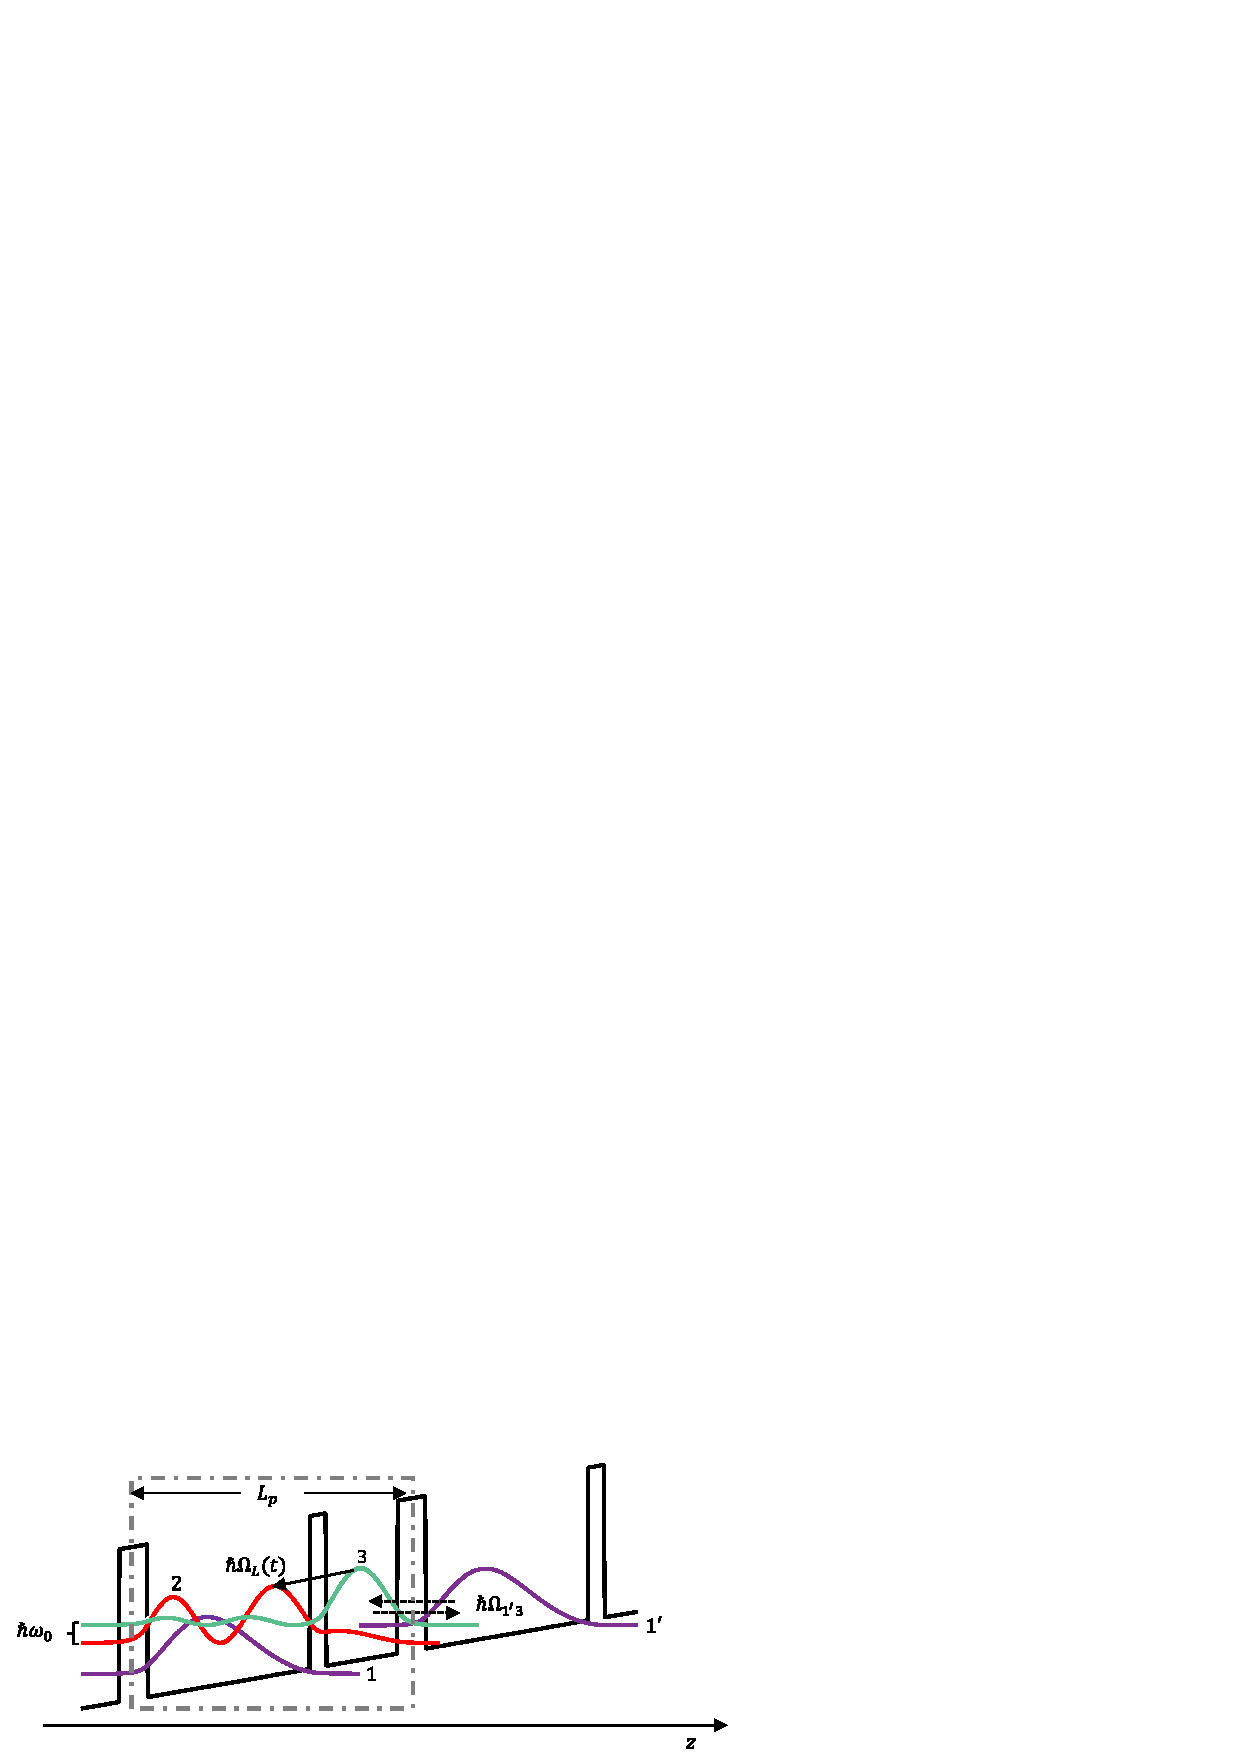
\includegraphics[scale=1]{img01.png}
\caption{Insert caption here} \label{fig:img01}
\end{figure}

Let us consider a simple three level resonant phonon QCL system as depicted in Fig. \ref{fig:img01}. In this configuration, there are four relevant laser levels $\Ket{1'}, \Ket{3}, \Ket{2} $ and $\Ket{1}$ which are the injector level, the upper and lower laser levels and the depopulation level, respectively. $\Ket{1'}$ couples to $\Ket{3}$ via the anticrossing energy $\hbar\Omega_{1'3}$, whereas the upper and lower laser levels interact via the optical Rabi frequency $\Omega_L(t)= \mu_{32}E_z(t)/\hbar$, where $\mu_{32} = -e \Bra{3}\hat{z} \Ket{2}$ is the dipole matrix element, $E_z(t)$ is the electric field component along the growth direction $z$ and $e$ is the elementary charge. Lastly, we assume that the energy separation between $\Ket{1'}$ and $\Ket{3}$ is $\Delta_{1'3} = \hbar \epsilon$ and that between the upper and lower laser levels $\Delta_{32} = \hbar \omega_0$.
The evolution of electron wave packets, cascading through the structure, are treated quantum mechanically within the density matrix formalism, where the equation of motion (EOM) is given by the von Neumann equation:
\begin{align}
 \label{eq:vonNeumann}
 i\hbar \frac{d \hat{\rho}}{dt} = [\hat{H};\hat{\rho}].
\end{align}
Above $\hat{\rho}$ denotes the density operator, $\hat{H}$ the Hamiltonian of the system, and $[\cdot;\cdot]$ the usual quantum mechanical commutator. In general, $\hat{H}$ contains many different contributions corresponding to various physical mechanisms that determine the overall carrier transport in the system. These could be radiative transitions or coherent and incoherent scattering events such as resonant tunneling for the former and LO phonon, electron-electron, interface roughness etc. for the latter. In principle, each scattering process enters Eq. (\ref{eq:vonNeumann}) via a corresponding potential operator $\hat{V}$. Time-stepping the Schrödinger equation when all of the above enumerated mechanisms are included is a daunting numerical task as it might involve additional discretization in $k-$space as well as the evaluation of complicated integrals (for time dependent potentials $\hat{V}(t)$). However, to simplify the equations at hand we  invoke first order time dependent perturbation theory and treat all incoherent scattering process within a rate equation approach, whereas only the coherent and radiative scattering mechanisms quantum mechanically. Due to the fact that resonant tunneling (to a first order approximation) conserves the wave vector ($\mathbf{k}$) of electrons, we can consider the density matrix components in position space representation \emph{only}, i.e. we can omit any dependence on the $\mathbf{k}$. Furthermore, the rates for each incoherent subband transition event are not chosen arbitrarily, but instead are calculated from Fermi's golden rule with our well established ensemble Monte Carlo simulation code[cite]. 

When resonant tunneling transitions are modelled, one usually employs the so called tight-binding approximation, where the wave functions are calculated for a single isolated period, whereas the electron subbands in adjacent modules are simply translated in space and energy by the module length $L_p$ [Q. Hu and Hallebaut]. However, the true time evolution of the system is still governed by the full or the extended Hamiltonian ($\hat{H}_{ext}$), consisting of multiple modules, so we need to compensate for the fact that we are using a tight-binding basis by including the correct anticrossing energies between levels spanning an intermodule barrier. In our case these are the injector and upper laser level whereas their coupling energy is assumed to be $\hbar \Omega_{1'3}$ (see Fig. \ref{fig:img01}). Finally, in this tight-binding basis, one can expand the von Neumann equation in matrix form as:
\begin{align}
 \label{eq:vonNeumannmatrix}
& i \hbar \frac{d}{dt} \begin{pmatrix}
\rho_{1'1'}& \rho_{1'3} & \rho_{1'2} \\
\rho_{31'} & \rho_{33} & \rho_{32} \\ 
\rho_{21'} & \rho_{23} & \rho_{22}
\end{pmatrix}  =  \left [ 
\overbrace{\begin{pmatrix} 
 \frac{\hbar \epsilon}{2} & \hbar\Omega_{1'3} & 0 \\
\hbar\Omega_{1'3}  & -\frac{\hbar	\epsilon}{2} &  \hbar\Omega_{L}(t) \\
0  &\hbar\Omega_{L}(t) & -\frac{\hbar \epsilon}{2}-\hbar\omega_{0}   
\end{pmatrix} }^{\text{resonant tunneling and radiative coupling}}
; 
\begin{pmatrix}
\rho_{1'1'}& \rho_{1'3} & \rho_{1'2} \\
\rho_{31'} & \rho_{33} & \rho_{32} \\ 
\rho_{21'} & \rho_{23} & \rho_{22}
\end{pmatrix}
\right ]  \nonumber \\
& + 
\underbrace{\begin{pmatrix}
	-\frac{\rho_{1'1'}}{\tau_{1'}} + (\frac{1}{\tau_{31'}}+\frac{1}{\tau_{31}})\rho_{33}  +  (\frac{1}{\tau_{21'}}+\frac{1}{\tau_{21}})\rho_{22} & \tau_{\parallel 1'3}^{-1}\rho_{1'3} & \tau_{\parallel 1'2}^{-1}\rho_{1'2}\\
   \tau_{\parallel 1'3}^{-1}\rho_{31'} & \frac{\rho_{1'1'}}{\tau_{1'3}}   - \frac{\rho_{33}}{\tau_{3}} +  \frac{\rho_{22}}{\tau_{23}} &  \tau_{\parallel 32}^{-1}\rho_{32}\\
   \tau_{\parallel 1'2}^{-1}\rho_{21'}& \tau_{\parallel 32}^{-1}\rho_{32} &	\frac{ \rho_{1'1'}}{\tau_{1'2}} + \frac{\rho_{33} }{\tau_{32}} 	- \frac{\rho_{22}}{\tau_2}
\end{pmatrix}}_{\text{scattering rates matrix}},
\end{align}
where $\rho_{i,j} = \Bra{i} \hat{\rho} \Ket{j}$ are the corresponding density matrix elements and we have set the zero energy at $E_0 = (E_{1'}+E_{3})/2 $. Also $\tau_{ij}^{-1}$ denotes the total outscattering rate from level $i$ to level $j$, $\tau_{i}$ the lifetime of level $i$ and
$$
	\tau_{\parallel ij}^{-1} = \frac{1}{2}(\frac{1}{\tau_{i}} +\frac{1}{\tau_{j}}) + \frac{1}{\tau_{pure}}   
$$
is the damping time of the coherence between levels $i$ and $j$, containing lifetime broadening and other "pure" dephasing mechanisms, which scramble the phase coherence between these subbands. 

Notice that in Eq. (\ref{eq:vonNeumannmatrix}) we have omitted the time evolution related to state $\Ket{1}$. This is due to the fact that the depopulation level, $\Ket{1}$, is effectively the injector level of the next period, which allows us to eliminate it from the model by employing "periodic" boundary conditions in the scattering rates matrix. It is vital for the simulation that these periodic boundary conditions are implemented correctly. This is so, because our model is formulated in a manner which does not contain phenomenologically included injection current density $J$ into the equations. Instead, we assume a periodic system where all carriers that reach the depopulation level $\Ket{1}$ are immediately re-injected into the system through level $\Ket{1'}$. In such a configuration the carrier number has to be conserved, which means that the relation $\sum_{j} d \rho_{jj}/dt =0 $ has to be satisfied at all times. Then, since the current injected into the system is essentially equal to the current entering into the depopulation level, from rate equation analysis we obtain that the current density is given by the formula:
\begin{equation}
\label{eq:currentdensity}
J = e L_p \left( \frac{\rho_{33}}{\tau_{31}} + \frac{\rho_{22}}{\tau_{21}} + \frac{\rho_{1'1'}}{\tau_{1'1}} \right)\approx e L_p \left( \frac{\rho_{33}}{\tau_{31}} + \frac{\rho_{22}}{\tau_{21}}  \right).  
\end{equation}
Note that this expression is similar to [Kumar], however it could be easily generalized for arbitrary number of levels via:
\begin{equation}
J = e L_p \left( \sum_{j=2}^{N}\frac{\rho_{jj}}{\tau_{j1}} + \frac{\rho_{1'1'}}{\tau_{1'1}} \right),
\end{equation}
where $\rho_{1'1'}$ denotes the injector level population and the $\rho_{jj}$ the density matrix elements corresponding to all electron transport "channel" levels within a single module.   


Since the density matrix has the Hermitian property, Eq. (\ref{eq:vonNeumannmatrix}) boils down to a system of six coupled ordinary differential equations for the unknowns $\rho_{1'1'}, \rho_{33},\rho_{22},\rho_{1'3},\rho_{32} $ and $\rho_{1'2}$. Expanded, Eq. (\ref{eq:vonNeumannmatrix}) takes the form:
\begin{subequations}
	\label{subeq:DM}
\begin{align}
\frac{d \rho_{1'1'}}{d t} &= i\Omega_{1'3} (\rho_{1'3} - \rho_{31'}) + (\frac{1}{\tau_{31'}}  + \frac{1}{\tau_{31}})\rho_{33} + (\frac{1}{\tau_{21'}}   +\frac{1}{\tau_{21}})\rho_{22} - \frac{\rho_{1'1'}}{\tau_{1'}} ,  \label{eq:vonNeumannexpandedstart}\\ 
\frac{d \rho_{33}}{d t}   &= i\Omega_{1'3} (\rho_{31'} - \rho_{1'3}) + i\frac{\mu_{32} E}{\hbar} (\rho_{32}-\rho_{23}) + \frac{ \rho_{1'1'}}{\tau_{1'3}} +
 \frac{\rho_{22}}{\tau_{23}} - \frac{\rho_{33}}{\tau_{3}},  \\
\frac{d \rho_{22}}{d t}   &=- i\frac{\mu_{32} E}{\hbar} (\rho_{32}-\rho_{23}) +\frac{\rho_{1'1'}}{\tau_{1'2}}  + \frac{\rho_{33}}{\tau_{32}} - \frac{\rho_{22}}{\tau_{2}} , \\
\frac{d \rho_{1'3}}{d t}  &= -i\epsilon\rho_{1'3} +i \Omega_{1'3}(\rho_{1'1'} - \rho_{33}) +i\frac{\mu_{32}E}{\hbar}\rho_{1'2} -\tau_{\parallel 1'3}^{-1}\rho_{1'3}, \\
\frac{d \rho_{32}}{d t}   &= -i\omega_{0}\rho_{32} +i \frac{\mu_{32}E}{\hbar}(\rho_{33}-\rho_{22}) -i\Omega_{1'3}\rho_{1'2} -\tau_{\parallel 1'2}^{-1}\rho_{1'2},   \\
\frac{d \rho_{1'2}}{d t}  &= -i(\epsilon+\omega_0)\rho_{1'2} +i\frac{\mu_{32}E}{\hbar}\rho_{1'3} -i\Omega_{1'3}\rho_{32} -\tau_{\parallel 32}^{-1}\rho_{32} . \label{eq:vonNeumannexpandedend}
\end{align}
\end{subequations}

One can easily verify that this system conserves the trace of the density matrix by calculating:
$$
\frac{d }{dt}Tr(\rho) = \sum_{j\in \{1',2,3\}} \frac{d \rho_{jj}}{dt} = 0.
$$

The essence of the Maxwell-Bloch equations is now in the couplig of the microscopic density matrix equations to the macroscopic Maxwell's equations. This is usually done via the incorporation of  polarization term in Maxwell's equations as the expectation value of the quantum mechanical dipole moment operator, i.e. :
\begin{equation} 
P_z = N\Gamma Tr\{\rho \mu\} = -N\Gamma(\mu_{32}\rho_{32} + \mu_{23}\rho_{23}) =  -N\Gamma\mu_{32}(\rho_{32}+\rho_{23}) , \label{eq:fullpolarization}
\end{equation}
where $N$ is the average carrier density per unit volume and $\Gamma$ is the spatial overlap between the optical field  and the active region. Assuming no free electric charges and also weak inhomogeneities in the polarization field, we obtain the classical wave equation for  $E_z$:
\begin{equation}
(\partial^2_{x} -\frac{n^2}{c^2}\partial^2_t) E_z = \frac{1}{\epsilon_0 c^2}\partial^2_t P_z, 
\label{eq:fullwave}
\end{equation}
where $x$ denotes the propagation direction, $c$ the speed of light in vacuum, $n$ is the refractive index of our material and $\epsilon_0$ is the permittivity of free space.

\subsection{Maxwell-Bloch equations for a Fabry-Perot resonator} 
The system of equations  (\ref{subeq:DM}) together with Eq. (\ref{eq:fullwave}) is a coupled non-linear system of ordinary and partial differential equations, which does not have known analytical solutions. This necessitates their numerical simulation on a computer, which however is still a difficult task since propagating the electric field in time, i.e. Eq. (\ref{eq:fullwave}), would require a very small grid size and correspondingly small time step and thus would take considerable computational power for long time simulations. In order to reduce the numerical effort, we will employ the rotating wave (RWA) and the slowly varying envelope approximations (SVEA) [give reference]. The optical field inside a Fabry-Perot cavity can be written as a superposition of forward and backward propagating waves as: 
\begin{align}
	E_z(x,t) &= \frac{1}{2} \big ( f_{+} e^{i(k_c x-\omega_c t)} + f_{-} e^{-i(k_c x+\omega_c t)} + c.c \big )\label{eq:sveaefield}
\end{align}
where "c.c." denotes the complex conjugate of the preceding expression, the $+$ and $-$ signs specify the forward/backward propagating waves' envelopes, respectively, and $\omega_c$  and $k_c$ are the field's  carrier frequency and wave number, related by $k_c = n \omega_c  / c$. Since the superposition of two counter propagating waves forms a standing wave, this will lead to the formation of an inversion grating along the propagation direction $x$, a phenomenon also known as spatial hole burning. Thus for the diagonal elements of the density matrix we make the following ansatz:
\begin{align}
      \rho_{ii}(x,t) = \rho_{ii}^0 + \rho_{ii}^+ e^{2ik_c x} + \rho_{ii}^-e^{-2ik_c x}, \label{eq:sveaansatz}
\end{align}
where $\rho_{ii}^+ = (\rho_{ii}^-)^*$ are the inversion grating's amplitudes. The ansatz in Eq. (\ref{eq:sveaansatz}) is justified since the population inversion follows the \emph{intensity} of the field and not its amplitude, from where it follows that the inversion grating ought to be proportional to $\propto sin(2k_cx)$ and not $sin(k_c x)$. Lastly, we decompose the coherences of the density matrix as:
\begin{align}
   \rho_{32} &= \eta_{32}^{+}e^{i(k_cx-\omega_ct)} + \eta_{32}^{-}e^{-i(k_c x+\omega_c t)}, \nonumber \\
   \rho_{1'2} &= \eta_{1'2}^{+}e^{i(k_c x - \omega_c t)} + \eta_{1'2}^{-}e^{-i(k_c x+\omega_c t)}, \nonumber \\
   \rho_{1'3} &= \rho_{1'3}^0 + \rho_{1'3}^{+} e^{2ik_cx} +  \rho_{1'3}^{-} e^{-2ik_cx}.   \label{eq:sveacoherences}
\end{align}
Notice that the term $\rho_{1'3}$ is assumed to evolve in a similar manner as the $\rho_{jj}$'s whereas $\rho_{32}$ and $\rho_{1'2}$ follow the electric field ansatz. Indeed, a simple exercise in change of basis shows us that $\rho_{1'3}$ can be expressed as:
\begin{equation}
\rho_{1'3} = \frac{1}{2}(\rho_{AA}-\rho_{SS}) + \frac{1}{2}(\rho_{SA}-\rho_{AS}), \label{eq:dressedrho}
\end{equation}
where $\rho_{AA} = \Bra{A}\hat{\rho}\Ket{A}$ ,$\rho_{SS} = \Bra{S}\hat{\rho}\Ket{S}$, $\rho_{SA} = \Bra{S}\hat{\rho}\Ket{A}$ and $\rho_{AS} = \Bra{A}\hat{\rho}\Ket{S}$   are the corresponding density matrix elements when we have changed into basis $\{\Ket{1'},\Ket{3},\Ket{2}\}\to\{\Ket{A},\Ket{S},\Ket{2}\}$, diagonalizing the submatrix of the Hamiltonian:
\begin{equation}
\hat{H}_{1'3} = \begin{pmatrix} 
\frac{\hbar \epsilon}{2} & \hbar\Omega_{1'3}  \\
\hbar\Omega_{1'3}  & -\frac{\hbar	\epsilon}{2} \\
\end{pmatrix} .
\end{equation}
In literature, the states $\Ket{S}$ and $\Ket{A}$ are also known as the symmetric and antisymmetric dressed states, eigenstates of $\hat{H}_{1'3}$, and in Eq. (\ref{eq:dressedrho}) we have assumed, for simplicity, that the detuning from resonance is $\hbar\epsilon \approx 0$.

Finally plugging in Eq. (\ref{eq:sveaefield}), (\ref{eq:sveaansatz}) and (\ref{eq:sveacoherences}) into Eq. (\ref{subeq:DM}), (\ref{eq:fullpolarization}) and (\ref{eq:fullwave})  and invoking the rotating wave and slowly varying amplitude approximations, we obtain our model in its final form.
\begin{subequations}
	\label{eq:finalthreelevelmodel}
\begin{align}
&\frac{n}{c}\partial_t f_{\pm} \pm \partial_{x}f_{\pm} = i\frac{N \Gamma \mu_{32} k_c}{\epsilon_0 n^2} \eta_{32}^{\pm} - \frac{l_0}{2} f_{\pm} \label{eq:rtwave} .\\
&\frac{d \rho_{1'1'}}{d t}^{0} = i\Omega_{1'3} (\rho_{1'3}^{0} - \rho_{31'}^{0}) + (\frac{1}{\tau_{31'}} + \frac{1}{\tau_{31}})\rho_{33}^{0} 
 + (\frac{1}{\tau_{21'}} + \frac{1}{\tau_{21}})\rho_{22}^{0} - \frac{\rho_{1'1'}^{0}}{\tau_{1'}} \\
&\frac{d \rho_{1'1'}}{d t}^{\pm} = i\Omega_{1'3} (\rho_{1'3}^{\pm} - \rho_{31'}^{\pm}) + (\frac{1}{\tau_{31'}} + \frac{1}{\tau_{31}})\rho_{33}^{\pm}  
+ (\frac{1}{\tau_{21'}} + \frac{1}{\tau_{21}})\rho_{22}^{\pm} - (\frac{1}{\tau_{1'}} + 4k_c^2D )\rho_{1'1'}^{\pm}  \label{eq:rtpop1grating}\\
&\frac{d \rho_{33}}{d t}^0 = i\Omega_{1'3} (\rho_{31'}^0 - \rho_{1'3}^0) + i\frac{\mu_{32}}{2\hbar} \big (f_{-}^*\eta_{32}^{-}+f_{+}^*\eta_{32}^{+} - c.c. \big )+ \frac{1}{\tau_{1'3}}\rho_{1'1'}^0 +  \frac{1}{\tau_{23}}\rho_{22}^0 - \frac{\rho_{33}^0}{\tau_{3}}  \\
&\frac{d \rho_{33}}{d t}^{+}   = i\Omega_{1'3} (\rho_{31'}^{+} - \rho_{1'3}^{+}) + i\frac{\mu_{32}}{2\hbar}\big ( f_{-}^*\eta_{32}^{+}-f_{+}(\eta_{32}^{-})^* \big ) 
+ \frac{\rho_{1'1'}^+}{\tau_{1'3}} +  \frac{\rho_{22}^+}{\tau_{23}} - (\frac{1}{\tau_{3}} +4k_c^2D) \rho_{33}^+ \label{eq:rtpop3grating}\\
&\frac{d \rho_{22}}{d t}^{0}  = -i\frac{\mu_{32}}{2\hbar} \big (f_{-}^*\eta_{32}^{-}+f_{+}^*\eta_{32}^{+} - c.c. \big ) + \frac{1}{\tau_{1'2}}\rho_{1'1'}^0  +  \frac{1}{\tau_{32}}\rho_{33}^{0} - \frac{\rho_{22}^0}{\tau_{21}} , \\
&\frac{d \rho_{22}}{d t}^{+}   = - i\frac{\mu_{32}}{2\hbar}\big ( f_{-}^*\eta_{32}^{+}-f_{+}(\eta_{32}^{-})^* \big )  + \frac{1}{\tau_{1'2}}\rho_{1'1'}^+  +  \frac{1}{\tau_{32}}\rho_{33}^+ - (\frac{1}{\tau_{2}}+4k_c^2D) \rho_{22}^+ , \label{eq:rtpop2grating}\\
&\frac{d \rho_{1'3}}{d t}^0  = -i\epsilon\rho_{1'3}^0 +i \Omega_{1'3}(\rho_{1'1'}^{0} - \rho_{33}^{0}) +i\frac{\mu_{32}}{2 \hbar}\big (f_{+}^*\eta_{1'2}^{+}+f_{-}^*\eta_{1'2}^{-} \big ) -
\tau_{\parallel 1'3}^{-1} \rho_{1'3}^{0} ,  \\
&\frac{d \rho_{1'3}}{d t} ^\pm = -i\epsilon\rho_{1'3}^\pm  +i\Omega_{1'3}(\rho_{1'1'}^{\pm} - \rho_{33}^{\pm}) +i \frac{\mu_{32}}{2 \hbar} f_{\mp}^* \eta_{1'2}^{\pm} 
- (\tau_{\parallel 1'3}^{-1} +4k_c^2 D)\rho_{1'3}^{\pm} ,\label{eq:rho13grating}\\
&\frac{d \eta_{32}^{\pm}}{d t}   = i(\omega_c - \omega_{0})\eta_{32}^{\pm} +i \frac{\mu_{32}}{2\hbar}\Big(  f_{\pm}(\rho_{33}^0-\rho_{22}^0) + f_{\mp}(\rho_{33}^\pm-\rho_{22}^\pm) \Big ) - i\Omega_{1'3}\eta_{1'2}^{\pm}
- \tau_{\parallel 32}^{-1}\eta_{32}^\pm , \\
&\frac{d \eta_{1'2}^\pm}{d t}  = i(\omega_c - \omega_{0}-\epsilon)\eta_{1'2}^{\pm} +i \frac{\mu_{32}}{2\hbar}(f_{\pm }\rho_{1'3}^0 + f_{\mp} \rho_{1'3}^{\pm}) - i\Omega_{1'3}\eta_{32}^{\pm} - \tau_{\parallel 1'2}^{-1}\eta_{1'2}^\pm.
\end{align}
\end{subequations}
Notice that in Eq. (\ref{eq:rtwave}) we have added, phenomenologically, a linear power loss coefficient $l_0$, and in equations (\ref{eq:rtpop1grating},\ref{eq:rtpop3grating} ,{\ref{eq:rtpop2grating},\ref{eq:rho13grating}) a diffusion term $4k_c^2D$ describing the diffusion rate at which carriers diffuse away from peaks of the population grating. Here $D$ denotes the diffusion constant, which for GaAs-AlGaAs systems is approximately 46 $cm^2/sec$ [cite].
\section{Applications}
\subsection{Extension of the model to multiple levels}
In this section we use our model for the numerical analysis of one of the best performing QCL based terahertz frequency combs so far, the active region from reference[]. This laser is based on a highly coherent resonant LO phonon gain medium, lasing at a central frequency of $f_0\approx 3.5 (THz)$, and  has been shown to produce a stable multimode spectrum containing more than 70 equidistant longitudinal modes in a free running regime of operation. At optimal biases, field autocorrelation measurements show a pulse-like periodic signal with a very strong and narrow beatnote with minimal reported FWHM linewidth of approximately 1.53 kHz. Furthermore, a novel comb coherence detection technique, SWIFT, was used to prove the stability of the terahertz comb over a large number of round trips. In what follows, we present an extensive analysis of the device within dynamic ranges where our modelling is applicable. We start off by wave function calculations in order to determine operating regimes where the "single resonant tunneling and single optical transition" assumption of our model could be applied. For these values of the bias, in [subsection] we conduct numerical experiments to calculate the spectrally resolved complex refractive index as well as to characterize the gain recovery of the device in question. In [subsection] we present time domain and spectral analysis of the transient dynamics of this laser for simulations exceeding many thousands of round trips.  

\begin{figure}[h!]
	\begin{center}
		\includegraphics[scale=.8]{img02b.png}
		\caption{Insert caption here} \label{fig:img02}
	\end{center}	
\end{figure}

Fig. \ref{fig:img02} \textbf{a)} illustrates the calculated wave functions for this device, when the tight binding approximation is employed. From graphical inspection we see that there are in total of five relevant levels per period, which we will refer to, according to their assumed role, as $\Ket{ULL}$ for the upper laser level, $\Ket{LLL1}$ for the higher energy level from a pair of lower laser levels, $\Ket{LLL2}$ for the lower energy level from the same pair, $\Ket{DEP1}$ for the higher energy level from a doublet of depopulation levels, and finally $\Ket{DEP2}$ for the lowest energy level. Furthermore, since the structure is periodic, the depopulation levels from the previous period will be referred to as $\Ket{INJ1}$ and $\Ket{INJ2}$, respectively.

Fig. \ref{fig:img02} \textbf{b)} and \ref{fig:img02} \textbf{c)} depict the calculated, for different biases, coupling strengths, $\hbar \Omega_{ij}$, between the injector states and the upper laser level as well as the dipole matrix elements, $\mu_{ij}$, between the upper laser level and the lower laser levels doublet. The anticrossing energies (AC) were calculated via the method described in [G.Bastard] and the numerical values were verified by diagonalization of the tight binding Hamiltonian. Our analysis shows that at biases around 9.2 kV/cm and 11 kV/cm there is an energetic resonance between $\Ket{INJ1} \leftrightarrow \Ket{ULL}$ and $\Ket{INJ2} \leftrightarrow \Ket{ULL}$, respectively, accompanied by a strong anticrossing energy coupling of the same levels. At and around those two operating regimes, the laser switches between a resonant tunneling $\Ket{INJ1}\leftrightarrow \Ket{ULL}$ transition for the former, and a resonant tunneling  $\Ket{INJ2} \leftrightarrow \Ket{ULL}$ transition for the latter. For example, at 11 kV/cm the wave functions $\ket{INJ2}$ and $\Ket{ULL}$ are at exact resonance, also illustrated in Fig. \ref{fig:img02} \textbf{a)}, whereas $\Ket{INJ1}$ and $\Ket{ULL}$ are separated by approximately $\Delta_{INJ1,ULL} \approx 4.3 \text{ meV}$ (not shown in the figure). Despite this, the coupling strengths $\hbar \Omega_{INJ1,ULL} \approx 1.18 \text{ meV}$ and $\hbar \Omega_{INJ2,ULL} \approx 1.38 \text{ meV}$ are comparable which leaves one wondering if it is in order to neglect one of the barrier couplings in our density matrix model. The figure of merit to consider is the tunneling times for both injection channels, which are given by [Williams Thesis]:
$$
T_{ij} = \frac{1+\Delta_{ij}^2\tau_{\parallel ij}^2}{2\Omega_{ij}^2\tau_{\parallel ij}}, 
$$ 
where $\Delta_{ij}$ is the detuning between levels $i$ and $j$ and the other parameters are as previously defined. Now, assuming equal dephasing times $\tau_{\parallel INJ1,ULL} = \tau_{\parallel INJ2,ULL} = \tau_{\parallel}\approx 0.4 \text{ ps}$, which are characteristic for THz QCLs [Williams Thesis], we obtain that:
$$
\frac{T_{INJ1,ULL}}{T_{INJ2,ULL}} = \left(1+\Delta_{INJ1,ULL}^2\tau_{\parallel}^2\right)\times \left(\frac{\Omega_{INJ2,ULL}}{\Omega_{INJ1,ULL}}\right)^2 \approx 5.7, 
$$ 
meaning that the majority of the tunneling electrons will prefer the $\Ket{INJ2} \leftrightarrow \Ket{ULL}$ resonant channel.

On the other hand, dipole moment calculations show us that $\mu_{ULL,LLL1} \approx 4.43 \text{ nm} \times e $ is more than ten times the value of $\mu_{ULL,LLL2} \approx 0.41 \text{ nm} \times e$. Therefore, the oscillator strength $f_{ULL,LLL1}$ will be hundred-fold higher than $f_{ULL,LLL2}$ from which it follows that around this regime of operation, we can safely choose the lower laser level, i.e. state $\Ket{2}$ in our equations, to be subband $\Ket{LLL1}$ from the system under investigation. Similarly, due to the discussion above, we can set the injector level in our reduced model, i.e. $\Ket{1'}$, to state $\Ket{INJ2}$. Finally, we can map $\Ket{3}$ to subband $\Ket{ULL}$ and include the effect of the rest of the electron transport channels, the set $ S_2 =  \{\Ket{INJ1},\Ket{LLL2}\}$, inside the scattering rates matrix, i.e. within a rate equations approach.

 Indeed, assuming there are no coherent or radiative interactions between subbands  $S_1  = \{\Ket{INJ2}, \Ket{[ULL]}, \Ket{LLL1}\}$ and those in $S_2$, we see that the coherent time evolution of the density matrix $\rho_{5lvl}$ is given by:
\begin{align}
i\hbar \dot{\rho}_{5lvl} =
\renewcommand\arraystretch{1.3} \left[ \left ( \begin{array}{c | c}
H_{S_1} & 0 \\ 
\hline 
0 & H_{S_2}
\end{array} \right) ; \left ( \begin{array}{c | c}
\rho_{S_1} & \rho_{S_1,S_2} \\ 
\hline 
\rho_{S_2, S_1} & \rho_{S_2}
\end{array} \right)
\right] = 
\left ( \begin{array}{c | c}
[H_{S_1};\rho_{S_1}] &(H_{S_1}-H_{S_2}) \rho_{S_1,S_2}  \\ 
\hline 
\rho_{S_2, S_1}(H_{S_2}-H_{S_1}) & \underbrace{[H_{S_2};\rho_{S_2}]}_{=0}
\end{array} \right) ,
\end{align}
where we have denoted with $\rho_{S_i}$ the density matrix elements corresponding to the levels in set $S_i$, with $\rho_{S_1,S_2} = \rho_{S_2,S_1}$ the coherence terms matrices resulting from interaction between levels in those sets, and similarly for the matrix elements of the Hamiltonian $\hat{H}_{TB}$. We can see that, unless we consider incoherent scattering events, the time evolution of $\rho_{S_1}$ is completely decoupled from any interaction with $\rho_{S_2}$, and also since in our model $H_{S_2}$ is assumed diagonal, the submatrix $\rho_{S2}$ remains constant in time. Therefore, the contributions to interactions between levels in $S_1$ and $S_2$ will be those originating from incoherent scattering mechanisms, which we can self-consistently include via the corresponding scattering rates, calculated with our EMC code.

 To conclude, after a careful parametric study of the active region from reference [], we argue that our "single optical and single resonant tunneling transition" Maxwell-Bloch model, presented in Eq. (\ref{eq:finalthreelevelmodel}), ought to give us a reasonable approximation to the full device, consisting of five relevant levels per period i.e. $S = \{\Ket{INJ1},\Ket{INJ2},\Ket{ULL},\Ket{LLL1},\Ket{LLL2}\}$. Furthermore, it has been shown that an extension of the three level model in Eq. (\ref{eq:finalthreelevelmodel}) to a five level one, can be done by treating the residual levels in $S_2$ within a rate equation formalism. 

\subsection{Numerical THz time-domain spectroscopy (THz-TDS)}
Terahertz time-domain spectroscopy (THz-TDS) is a pump-probe spectroscopic technique, where a broadband THz pulse illuminates the sample under investigation and the resulting, post-interaction, optical field is combined with a much shorter reference laser pulse, before entering a detector. The detector's response is then recorded and the whole procedure is repeated while varying the delay of the reference pulse, thus allowing one to time-resolve the amplitude and phase of the original THz electric field. In the area of QCLs, THz-TDS is mostly used for gain characterisation and dispersion measurements of different active regions, where a weak THz pump pulse is injected into the gain medium, and consecutively detected, in the manner outlined above, after having propagated for several round trips inside the laser's cavity [Jukam, Burghoff]. 

In the same context, we use our model Eq. (\ref{eq:finalthreelevelmodel}) to simulate THz-TDS experiments on the active region from reference [], which will allow us to numerically calculate the spectrally resolved real and imaginary parts of the refractive index and from there relevant quantities such as the spectral gain, the group velocity, group velocity dispersion and others. In its essence, our simulation experiment is the same as the THz-TDS technique and is illustrated in Fig. \ref{fig:img03}. Neglecting spatial hole burning effects, which are not expected to play a vital role during the duration of the simulation experiment, we consider our model applied to a ring cavity laser, in which we let a weak un-chirped Gaussian pulse propagate for several round trips. At each time step $t_n$ of our simulation, as well as at different points along the cavity length $x_j$, we record the electric field envelope $f_j^{n}$ to finally obtain a digital signal for further data processing. From there, the real and imaginary parts of the refractive index can then be calculated in a straightforward manner, as briefly discussed below. 

\begin{figure}[h!]
	\begin{center}
		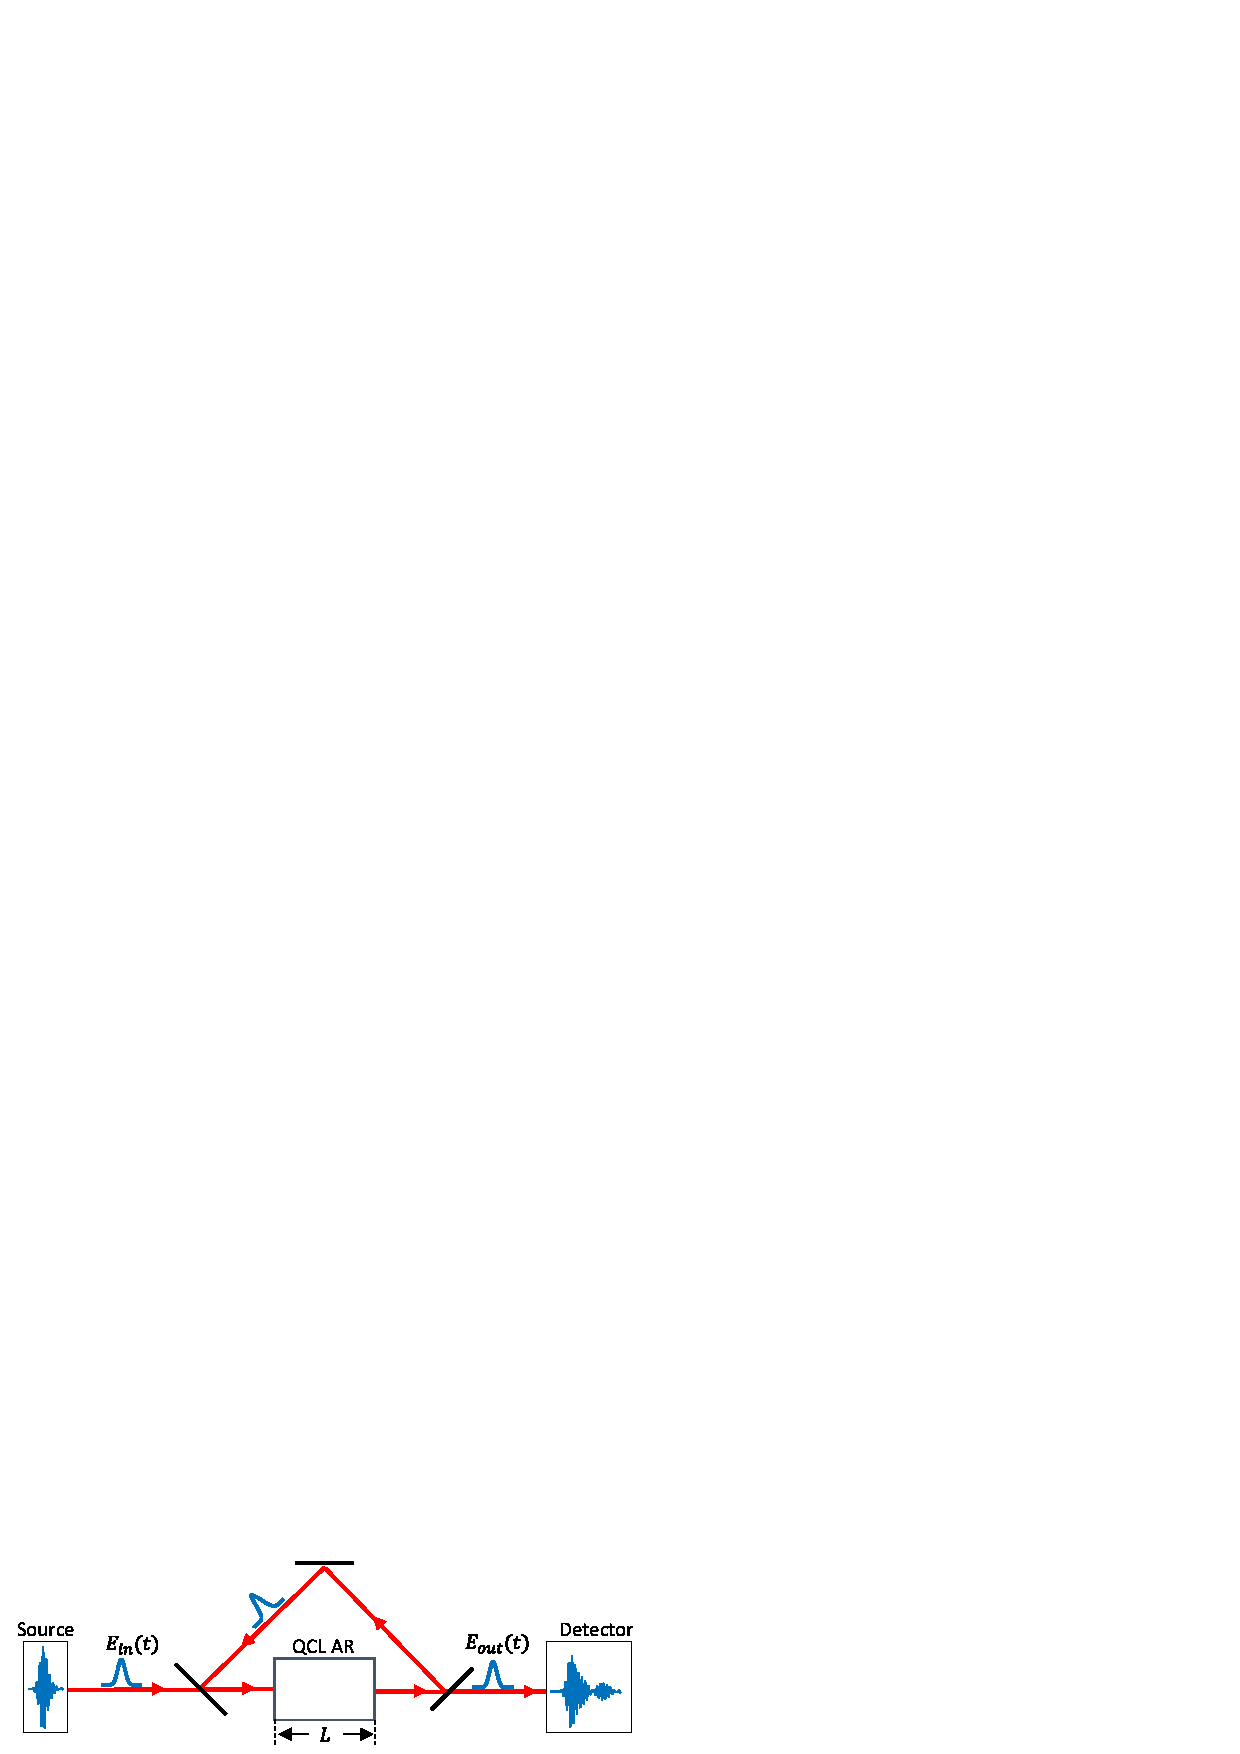
\includegraphics[scale=1.1]{img03.png}
		\caption{Insert caption here} \label{fig:img03}
	\end{center}	
\end{figure}

Let us first assume that some optical filed $E_{in}(t)$ traverses the dispersive cavity of length $L$ once. Let $E_{in}(\omega)$ and $E_{out}(w)$ be the Fourier transforms (FT) of the input and output signals $E_{in}(t)$ and $E_{out}(t)$, respectively. The question to investigate is how can we calculate the refractive index of the dispersive medium, given $E_{in}(t)$ and $E_{out}(t)$. Furthermore, since Eq. (\ref{eq:finalthreelevelmodel}), has been derived with respect to the \emph{envelope} of the electric field, we will need to reformulate all the calculations below in terms of this complex valued function. 

In a ring cavity, we have only forward propagating waves (no standing waves) and thus the electric field can be written as:
\begin{equation}
E(t,x) = \Re\{f(t,x)e^{i (k_c x - \omega_c t) }\} = \frac{1}{2} \left ( f(t,x)e^{i (k_c z - \omega_c t)} +f^*(t,x) e^{-i (k_c z - \omega_c t) }\right) ,
\end{equation}
where $f(t,x)$ is the (slowly varying) envelope function. Fourier transforming the above equation using the physics convention, we obtain:
\begin{equation}
E(\omega,x) = \frac{1}{2} \left( F(\omega-\omega_c)e^{ik_cx} +  F^*(-\omega-\omega_c)e^{-ik_cx} \right), 
\end{equation}
where $F(\omega)$  is the phasor of $f(t,x)$, corresponding to frequency component $\omega$.

Now, to obtain the real part of the refractive index we need to find out how much phase did $E_{out}(\omega)$ acquire after propagating a distance $L$ through the cavity. Well, we can write it down:
\begin{equation}
E_{out}(t,L)  = \frac{1}{2\pi} \int \underbrace{E_{in}(\omega) e^{i\Psi(\omega)}}_{E_{out}(\omega)}e^{-i\omega t}  d\omega,
\end{equation}
where $\Psi(\omega) = k(\omega)L$ is the total accumulated phase for angular frequency component at $\omega$ and $k(\omega)$ is the frequency dependent wave number. Therefore calculating the spectral phase $\Psi(\omega)$, boils down to:
\begin{equation}
\label{eq:phaseanglefield}
\Psi(\omega) = angle\{E_{out}(\omega)/E_{in}(\omega)\} = angle\{E_{out}(\omega) \} - angle\{E_{in}(\omega)\}.
\end{equation}
However, as mentioned above, we need to derive Eq. (\ref{eq:phaseanglefield}), in terms of expressions including the Fourier transform of the \emph{envelope}, $F(\omega)$. This is straightforward. If we assume that the bandwidth of $F(\omega)$ is narrow (i.e. that $F(\omega-\omega_c)$ and $ F^*(-\omega-\omega_c)$ do not overlap in frequency space), we can take only the positive frequency components and compare their phases, i.e. 
\begin{align}
\Psi(\omega) = angle\{E_{out}(\omega)/E_{in}(\omega)\} &= angle\{F_{out}(\omega-\omega_c)e^{ik_cL}/F_{in}(\omega-\omega_c)\}, \nonumber \\
& = angle\{F_{out}(\omega-\omega_c)/F_{in}(\omega-\omega_c)\} + k_cL. 
\end{align}
Denoting with 
\begin{equation}
\tilde{\Psi}(\tilde{\omega}) = angle\{F^*_{out}(\tilde{\omega})/F^*_{in}(\tilde{\omega})\}
\end{equation}
the phase difference between the envelope's spectral components, we get:
\begin{equation}
\label{eq:phaserelation}
\Psi(\tilde{\omega}+\omega_c) = \tilde{\Psi}(\tilde{\omega}) + k_cL,
\end{equation}
where we have set $\tilde{\omega} = \omega - \omega_c$. Now, to compute the real part of the refractive index $n'(\omega)$, we notice that:
\begin{equation}
\label{eq:wavenumberphase}
k(\omega)L = \Psi(\omega),
\end{equation}
and also that
\begin{equation}
\label{eq:wavenumberrefractiveidx}
k(\omega) =  \frac{n'(\omega)\omega}{c}.
\end{equation}
Combining Eq. ( \ref{eq:wavenumberphase}) and Eq. (\ref{eq:wavenumberrefractiveidx}) into Eq. (\ref{eq:phaserelation}), we finally obtain:
\begin{equation}
n'(\tilde{\omega}+\omega_c) = \frac{c}{(\tilde{\omega}+\omega_c)L}\tilde{\Psi}(\tilde{\omega})+\frac{ck_c}{(\tilde{\omega}+\omega_c)} = \frac{c}{(\tilde{\omega}+\omega_c)L}\tilde{\Psi}(\tilde{\omega}) +n\times\frac{ \omega_c}{(\tilde{\omega}+\omega_c)},
\end{equation}
with $n$ being the refractive index at the central frequency $\omega_c$ (i.e. $k_c = \omega_c n/c$). 

Similarly we can calculate the imaginary part of the refractive index by assuming that the accumulated phase can be a complex number. Then, the spectral gain $g(\omega)$ is simply given by the log of the ratio of the corresponding frequency components of the output and the input signals:
\begin{equation}
g(\tilde{\omega}+\omega_c) = \frac{1}{L} \log\{|F_{out}(\tilde{\omega})|/|F_{in}(\tilde{\omega})|\}.
\end{equation}
Since $g(\omega)$ can be related to the complex refractive index $n''(\omega)$ via:
\begin{equation}
g(\omega) = -\frac{n''(\omega)\omega}{c}, 
\end{equation}
this gives us:
\begin{equation}
n''(\tilde{\omega}+\omega_c) = -\frac{c}{(\tilde{\omega}+\omega_c)}\frac{1}{L} \log\{|F_{out}(\tilde{\omega})|/|F_{in}(\tilde{\omega})|\}.
\end{equation}

\end{document}
